
% ------------------------------------------------
% --- INTRODUCTION -------------------------------
% ------------------------------------------------

\chapter{Introduction} \label{cha:introduction}

\emph{Network-centric operations} involve multiple agents that cooperate to achieve common goals. This can also be thought of as a \emph{system of systems} problem. A network-centric battle scene is depicted in Figure~\ref{fig:intro:network-centric-battle-scene}. We see multiple agents, \eg, manned and unmanned aircraft and vessels, ground vehicles, and command \& control. These platforms use local \emph{sensors}, \eg, radar and imaging systems, to extract information about targets. The sensor measurements are processed locally in \emph{processing units}, \eg, Kalman filters, where \emph{target estimates} are computed. In target tracking these estimates are often referred to as \emph{tracks}. The agents are also connected using a \emph{datalink} which provides means for sharing local information, \eg, the local tracks. 

\begin{figure}[bth]
	\centering
	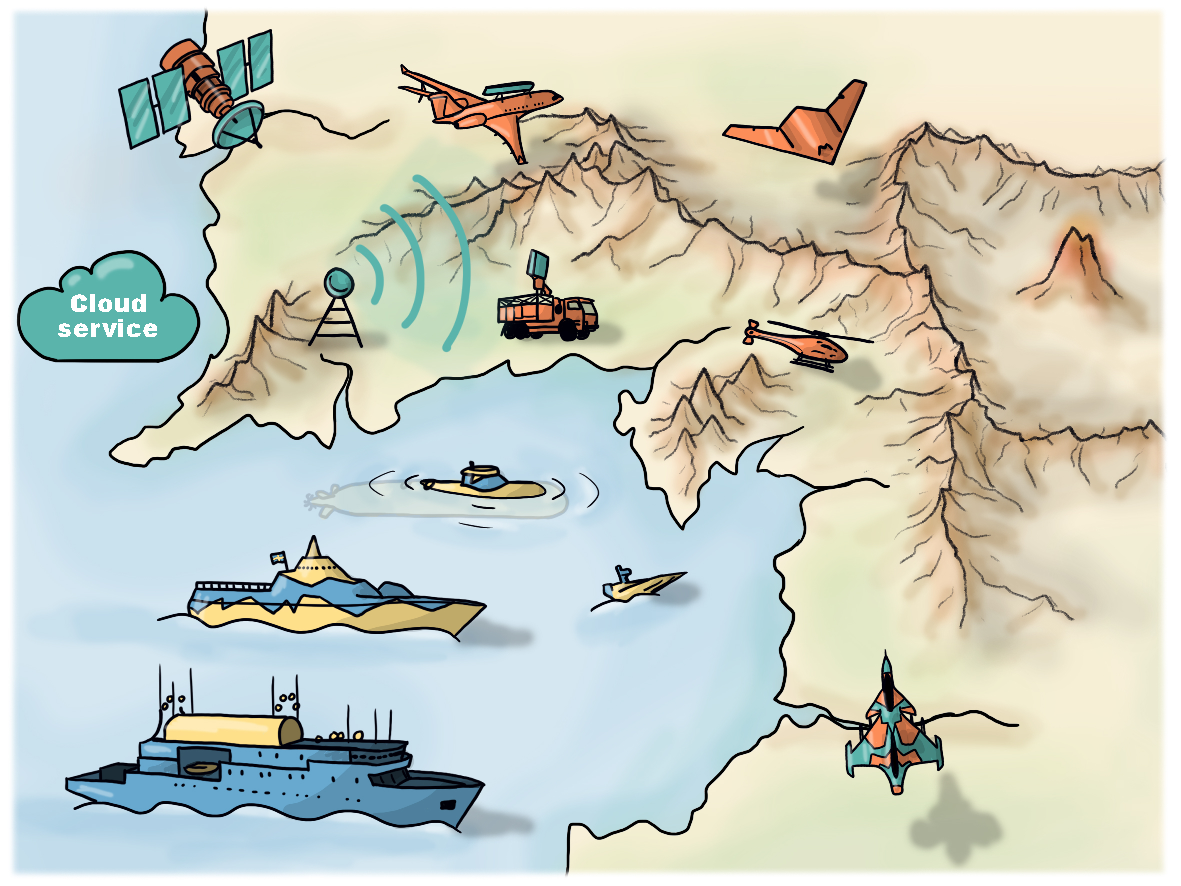
\includegraphics[width=.9\textwidth]{fig/cha1/network-centric_battle-scene.pdf}
	\caption{A network-centric battle scene. Multiple agents, both manned and unmanned, of different classes, \eg, ground vehicles, ground stations, aircraft, and ships, use onboard sensor to extract information. The information is then shared among the agents over a datalink for improved situation awareness and decision-making. }
	\label{fig:intro:network-centric-battle-scene}
\end{figure}




% --- NETWORK-CENTRIC TARGET TRACKING ---
\section{Target Tracking in Sensor Networks}

One crucial benefit of network-centric \emph{target tracking} is the information sharing which allows for improved tracks to be obtained. By utilizing \emph{data fusion} techniques local tracks can be fused with tracks received over the datalink. However, for the data fusion to work properly care must be taken regarding which method is being used for track fusion. In particular, the uncertainty assessment is important. Some methods might compute a too small uncertainty which makes the fused track not trustworthy. Other methods might compute a too large uncertainty such that the fused track becomes useless. Which method to use is essentially a design choice but depends on factors such as the network design, communication pattern, and processing units being used.

The networks considered here are \emph{sensor networks}. A sensor network consists of sensor nodes and processing unit nodes with edges resembling the datalink. In the next we will discuss some crucial aspects of target tracking in sensor networks.


% SN ARCHITECTURE
\subsection{Sensor Network Design}

The price paid when using multiple sensor and processing units is increased complexity in terms of computations, communication, and system design. How and to what extent the complexity is increased depends on the network design. In a \emph{centralized sensor network}, see Figure~\ref{fig:intro:centralized}, all sensors communicate their measurements to a central processing unit. This arrangement allows for optimal target tracking performance but suffers from high communication demands and single points of failure. Hence, a centralized sensor network is not suitable for critical applications such as the one depicted in Figure~\ref{fig:intro:network-centric-battle-scene}.

\begin{figure}[tb]
	\centering
	\begin{subfigure}[b]{0.475\columnwidth}
		\centering
		\begin{tikzpicture}[scale=.1]
			
\def\rf{1.5}
\def\rs{1}

\def\xf{0}
\def\yf{0}


% --- FIGURE ---
\draw [white,opacity=.0] (-30,-5) rectangle (30,5);

\foreach \x/\y in {-10/-11,2/-12,-18/-2,17/-5,20/-1,19/10,7/9,-9/12,-17/8,-19/3} {
	\drawsensorarrow[shorten >=5] (\x,\y) -- (\xf,\yf);
	\drawsensornode (\x,\y) circle [radius=\rs]; 
}

\drawprocessingunit{clra} (\xf,\yf) circle [radius=\rf];
		\end{tikzpicture}
		\caption{Centralized sensor network}
		\label{fig:intro:centralized}
	\end{subfigure}
	%
	\begin{subfigure}[b]{0.475\columnwidth}
		\centering
		\begin{tikzpicture}[scale=.1]
			
\def\rf{1.5}
\def\rs{1}

\def\xf{0}
\def\yf{0}

\def\xfa{1}
\def\yfa{-7}

\def\xfb{-10}
\def\yfb{-3}

\def\xfc{-8}
\def\yfc{11}

\def\xfd{15}
\def\yfd{9}

\def\xfe{16}
\def\yfe{-7}

\def\xff{-8}
\def\yff{-12}

\def\shortenlength{5}



% --- FIGURE ---
\draw [white,opacity=.0] (-30,-5) rectangle (30,5);


% Sensor nodes
\foreach \x/\y in {-24/-3,-22/-6,-19/-9} {
	\drawsensorarrow[shorten >=\shortenlength] (\x,\y) -- (\xfb,\yfb);
	\drawsensornode (\x,\y) circle [radius=\rs]; }

\foreach \x/\y in {-18/15} {
	\drawsensorarrow[shorten >=\shortenlength] (\x,\y) -- (\xfc,\yfc);
	\drawsensornode (\x,\y) circle [radius=\rs]; }

\foreach \x/\y in {21/14} {
	\drawsensorarrow[shorten >=\shortenlength] (\x,\y) -- (\xfd,\yfd);
	\drawsensornode (\x,\y) circle [radius=\rs]; }

\foreach \x/\y in {25/-6, 25/-9} {
	\drawsensorarrow[shorten >=\shortenlength] (\x,\y) -- (\xfe,\yfe);
	\drawsensornode (\x,\y) circle [radius=\rs]; }

%\foreach \x/\y in {-15/-20} {
%	\drawsensorarrow[shorten >=5] (\x,\y) -- (\xff,\yff);
%	\drawsensornode (\x,\y) circle [radius=\rs]; }


% Fusion nodes and communication lines
\foreach \x/\y/\c in {\xfa/\yfa/clra,\xfb/\yfb/clrb,\xfc/\yfc/clrc,\xfd/\yfd/clrd,\xfe/\yfe/clre} {
	\drawprocessingunit{\c} (\x,\y) circle [radius=\rf]; } % ,\xff/\yff/clrf

\drawcomarrow [<->,shorten >=\shortenlength,shorten <=\shortenlength] (\xfa,\yfa) -- (\xfb,\yfb);
\drawcomarrow [<->,shorten >=\shortenlength,shorten <=\shortenlength] (\xfa,\yfa) -- (\xfc,\yfc);
\drawcomarrow [<->,shorten >=\shortenlength,shorten <=\shortenlength] (\xfb,\yfb) -- (\xfc,\yfc);
\drawcomarrow [->,shorten >=\shortenlength,shorten <=\shortenlength] (\xfc,\yfc) -- (\xfd,\yfd);
\drawcomarrow [<->,shorten >=\shortenlength,shorten <=\shortenlength] (\xfd,\yfd) -- (\xfe,\yfe);
%\drawcomarrow [<->,shorten >=\shortenlength,shorten <=\shortenlength] (\xfe,\yfe) -- (\xff,\yff);
\drawcomarrow [<-,shorten >=\shortenlength,shorten <=\shortenlength] (\xfa,\yfa) -- (\xfe,\yfe);
%\drawcomarrow [<->,shorten >=\shortenlength,shorten <=\shortenlength] (\xfb,\yfb) -- (\xff,\yff);
		\end{tikzpicture}
		\caption{Decentralized sensor network}
		\label{fig:intro:decentralized}
	\end{subfigure}
	%
	\caption{Sensor networks. Black and colored circles resemble sensor nodes and processing units, respectively. The solid and dotted arrows illustrate sensor-to-processing unit and inter-processing unit communication, respectively.} 
	\label{fig:bkg:sn}
\end{figure}

The focus in the thesis is target tracking in \emph{decentralized sensor networks} (DSNs). A \abbrDSN is illustrated in Figure~\ref{fig:intro:decentralized}. This type of network is, \eg, realized by wireless ad hoc networks such as wireless sensor networks \cite{Toh1997WANET}. According to \cite{Grime1994CEP}, a \abbrDSN is characterized by the following properties:
\begin{enumerate}[label=C\arabic*]
	\item There is no single point of failure. Failure of one node of the network does not cause a complete network breakdown.
	\item There is no central communication management system. Nodes can, in general, only communicate on a node-to-node basis.
	\item There is no global knowledge about the network topology locally available at the nodes.
\end{enumerate}

In a \abbrDSN, measurements are passed to a local processing unit, where local tracks are computed. The local tracks are then exchanged between the processing units to enhance the tracking quality by fusion. A decentralized design yields the following advantages over a centralized counterpart \cite{Julier2009-ch14,Uhlmann2003IF}:
\begin{itemize}
	\item \emph{Robustness}. Since there is no single point of failure, a decentralized design is inherently fault-tolerant. 
	\item \emph{Modularity}. The network is decomposed into smaller, self-contained subsystems, which reduces the overall complexity and makes the network scalable. This also makes the system design process easier since these components can be developed and maintained separately.
	\item \emph{Flexibility}. It is possible to connect, update, and disconnect the self-contained subsystems on-the-fly.
\end{itemize}
These properties are vital for the scene illustrated in Figure~\ref{fig:intro:network-centric-battle-scene}.

\begin{remark}
A \abbrDSN is an example of distributed processing. However, the terms decentralized and distributed should not be used interchangeably. While distributed sensor networks have multiple interconnected processing units, there is typically a central coordinator or some global processing result is obtained, \eg, globally available tracks \cite{Castanedo2013TSWJ}. This work is limited to methods that are able to cope with the constraints imposed by C1--C3, thereby excluding many distributed processing techniques. On the contrary, decentralized methods are typically applicable in distributed processing problems.
\end{remark}




% PROCESSING UNITS
\subsection{Decentralized Target Tracking}

Data association and state estimation are fundamental components of the processing unit within a target tracking system. The data association involves the assignment of measurements to tracks, which often requires solving an optimization problem in order to identify the optimal pairings between measurements and tracks based on a specified cost function. In state estimation, the tracks are updated by incorporating the assigned measurements. The existing body of literature pertaining to target tracking, particularly in a centralized setting, is extensive, with numerous publications dedicated to this topic. However, in the context of DSNs, there remains a considerable amount of work to be undertaken to properly address the specific issues that arise in \emph{decentralized target tracking} (\abbrDTT).

Figure~\ref{fig:intro:dtt-system} provides a schematic view of the processing unit in a \abbrDTT system which contains the following functional components:
\begin{enumerate}
	\item \emph{Measurement-to-track association.} Assigns measurements to the local tracks.
	\item \emph{State estimation.} Updates local tracks with the assigned measurements.
	\item \emph{Track-to-track association.} Assigns local tracks to the received tracks. 
	\item \emph{Track fusion.} Fuses local tracks with the assigned tracks.
	\item \emph{Communication management.} Decides which track information to exchange.
\end{enumerate}
These functions are run recursively. The dashed line in Figure~\ref{fig:intro:dtt-system} illustrates that local tracks are predicted and used in the next time step. Roughly speaking, a centralized target tracking system involves steps 1--2 but not steps 3--5.

\begin{figure}[t]
	\centering
	\begin{tikzpicture}[scale=.9]
		


% --- FIGURE ---
\begin{scriptsize}

%\draw [white,opacity=.0] (0,-1) rectangle (17,0);

\drawprocessingunitbox{clra!40!} (2.75,-1.75) rectangle (14.75,2);
\node [below,font=\bfseries] at (8.75,2) {processing unit};

% STATE EST
\drawsensorbox (0,0) rectangle (2,1) node [pos=.5,font=\bfseries,color=white] {sensors};
\drawsystemarrow (2,0.5) -- (3,0.5);
\drawsystembox (3,0) rectangle (7,1) node [pos=.5,font=\bfseries,align=center] {measurement-to-track \\ association};
\drawsystemarrow (7,0.5) -- (8,0.5);
\drawsystembox (8,0) rectangle (10.5,1) node [pos=.5,font=\bfseries,align=center] {state \\ estimation};
\drawsystemarrow (9.25,0) -- (9.25,-0.25) -- (5,-0.25) -- (5,-0.5);

% FUSION
\drawsensorbox (0,-0.5) rectangle (2,-1.5) node [pos=.5,font=\bfseries,align=center,color=white] {datalink};
\drawsystemarrow (2,-1) -- (3,-1);
\drawsystembox (3,-0.5) rectangle (7,-1.5) node [pos=.5,font=\bfseries,align=center] {track-to-track \\ association};
\drawsystemarrow (7,-1) -- (8,-1);
\drawsystembox (8,-0.5) rectangle (10.5,-1.5) node [pos=.5,font=\bfseries,align=center] {track \\ fusion};

% COM
\drawsystemarrow (10.5,-1) -- (11.5,-1);
\drawsystemarrow [densely dashed] (10.75,-1) -- (10.75,1.25) -- (5,1.25) -- (5,1);
\draw [black,fill=black] (10.75,-1) circle [radius=0.05];
\drawsystembox (11.5,-0.5) rectangle (14.5,-1.5) node [pos=.5,font=\bfseries,align=center] {communication \\ management};
\drawsystemarrow (14.5,-1) -- (15.5,-1) node [near start,above right,align=center,font=\it] {exchanged \\ tracks};

\end{scriptsize}
	\end{tikzpicture}
	\caption{A decentralized target tracking system. }
	\label{fig:intro:dtt-system}
\end{figure}

\begin{remark}
There are other ways to model a DTT system than the functional breakdown of Figure~\ref{fig:intro:dtt-system}. For instance, basically all target tracking systems contain some track management logic, which is excluded here. It should, however, be noted that there is no distinct generic model used to illustrate every target tracking system. In the current scope, the model in Figure~\ref{fig:intro:dtt-system} is sufficiently rich.
\end{remark}

\begin{remark}
The operation governing the track fusion is often also referred to as data fusion or sensor fusion.
\end{remark}

The DSNs considered here are modeled as a network of agents. Each agent typically has one or several sensors, but in some cases none. Moreover, each agent comprises a self-contained target tracking system and a communication system. The agent can operate on its own under constraints C1--C3 and independently of the other agents.




% CORRELATIONS
\subsection{Correlations}

The essence of Figure~\ref{fig:intro:network-centric-battle-scene} is the huge amount of data that is transferred. Tracks and other estimates are exchanged between agents and further processed. This results in dependencies, \ie, the tracks become correlated with each other. For small, simple networks, the correlations might be tractable. However, in general, it is impossible to maintain explicit knowledge about these correlations among all agents. The issue of having only partial knowledge about correlations is a fundamental aspect of \abbrDTT.

In the scope of this thesis, a track is specified by a vector and a covariance matrix. These are the quantities that are being exchanged between agents for track fusion. Simply neglecting the correlations generally leads to undesirable results where the actual covariance matrix of a fused track is underestimated. In the worst case, tracks start to diverge due to incorrect uncertainty assessment \cite{Julier2009-ch14}. To avoid this, the notion of \emph{conservativeness} has been introduced. A conservative estimator is able to guarantee that the computed covariance matrix is no smaller than the covariance matrix of the actual error. 




% COMMUNICATION
\subsection{Communication}

Another crucial aspect of \abbrDTT problems is communication constraints \cite{Razzaque2013ACM}. State estimates and covariance matrices need to be communicated for a legion of targets and to and from many agents. At some point, the communication link will become a bottleneck, and hence the finite size of the communication resource must be taken into account. There are also situations where the communication needs to be reduced for other reasons, \eg, to be able to operate with a low electromagnetic signature. Hence, there is a need to study \abbrDTT under communication constraints \cite{Kimura2005ITCC}.





% --- PROBLEM ---
\section{Problem Statement} \label{sec:intro:problem-statement}

The main goal of the thesis is to increase the performance and usability of \abbrDTT systems. The research focus is related to the \emph{track fusion} and \emph{communication management} components of Figure~\ref{fig:intro:dtt-system}. In particular, the following two subproblems are addressed:
\begin{enumerate}[label=P\arabic*]
	\item Robust track fusion under unknown correlations. To be useful, the track fusion needs to consider both conservativeness and tracking performance.
	\item Efficient usage of the communication resource. The main design criteria for the communication management are the amount of communicated data, conservativeness, and tracking performance.
\end{enumerate}





% --- SCOPE ---
\section{Scope}

The scope of this report slightly differs from the thesis. The report takes a more practical approach. In particular, we will focus on: (i) the evaluation of track fusion design; and (ii) how to implement the communication management. (i) and (ii) are related to P1 and P2, respectively.

Many of the theoretical considerations of the thesis are excluded here. We also assume a single-target tracking environment and that the data association process can be ignored.



% --- REPORT OUTLINE ---
\section{Report Outline}

This report is organized as follows:

Chapter~2 deals with the track fusion design and evaluation in the single-target tracking case. Three commonly adopted track fusion methods are presented. Several important evaluation measures are defined. The track fusion methods are analyzed using the considered evaluation measures.

Chapter~3 deals with \abbrDTT under communication constraints. Methods for preserving conservativeness under certain communication constraints are proposed. We define and discuss a framework for reducing dimensionality for optimal track fusion performance. A resolution is proposed to the problem of only having access to local information when reducing dimensionality.

Chapter~4 concludes this report and specifies which parts of the thesis that are not included here.




% --- SOURCE CODE ---
\section{Source Code Accessibility} \label{sec:intro:source-code} 

\matlab source code related to the thesis is publicly accessible at \githuburl. This includes the source code for all numerical evaluations and all examples where it is applicable. The repository also contains a \abbrDTT simulation environment that can be adapted for testing and evaluating new theory and algorithms.



